\documentclass[a4paper, amsfonts, amssymb, amsmath, reprint, showkeys, nofootinbib, twoside]{revtex4-1}
\usepackage[spanish]{babel}
\usepackage[utf8]{inputenc}
\usepackage{float}
\usepackage[colorinlistoftodos, color=green!40, prependcaption]{todonotes}
\usepackage{amsthm}
\usepackage{mathtools}
\usepackage{physics}
\usepackage{xcolor}
\usepackage{graphicx}
\usepackage[left=23mm,right=13mm,top=35mm,columnsep=15pt]{geometry} 
\usepackage{adjustbox}
\usepackage{placeins}
\usepackage[T1]{fontenc}
\usepackage{lipsum}
\usepackage{csquotes}
\usepackage[normalem]{ulem}
\useunder{\uline}{\ul}{}
\usepackage[pdftex, pdftitle={Article}, pdfauthor={Author}]{hyperref} % For hyperlinks in the PDF
%\setlength{\marginparwidth}{2.5cm}
\bibliographystyle{apsrev4-1}

\begin{document}

%El título del experimento realizado es importante.
\title{Figuras de Lissajous}


\author{Carlos Mauricio Devia Zorro}
\email[Correo institucional: ]{cm.devia@uniandes.edu.co}

%Si necesitan poner un segundo autor, deben eliminar los porcentajes (%) iniciales.
  
\author{Sergio Montoya Ramírez}
\email[Correo institucional: ]{s.montoyar2@uniandes.edu.co}

\affiliation{Universidad de los Andes, Bogotá, Colombia.}

\date{\today} % Si lo dejan vacío no les saldrá fecha. La fecha que se muestra es del día en que se compila.

\begin{abstract}

    Las figuras de Lissajous son formas que surgen de la intersección de dos ondas en donde una se encarga de las coordenadas en el eje x y la otra de las coordenadas en el eje y. En este experimento, se construyen algunas figuras de Lissajous basicas por medio de un osciloscopio, un generador y un computador.

\end{abstract}

\maketitle

\section{Objetivos}
\begin{itemize}
  \item Entender el funcionamiento del osciloscopio y el generador de señales periodicas.
  \item Importar imágenes a \textit{Logger Pro} por medio del software que controla el osciloscopio.
  \item Determinar la relación entre la forma de la figura de Lissajous y la amplitud, frecuencia y diferencia de fase entre dos oscilaciones.
\end{itemize}
\section{Introducción}

Un movimiento Ondulatorio puede expresarse con funciones trigonometricas. Sin embargo, cuando se combinan dos ondulaciones que varian en frecuencia y fase inicial emergen figuras de mucho interes. Estas figuras, se llaman figuras de Lissajous \cite{French}. El objetivo de este laboratorio es que el estudiante se familiarice con estas figuras

\section{Montaje experimental}

\subsection{Materiales}
\begin{itemize}
    \item Osciloscopio TBS 1102B-EDU.
    \item Generador de señales AFG1022.
    \item Dos sondas BNC - BNC.
    \item Sonda Osciloscopio.
    \item Cable USB A a USB B para conexión del osciloscopio al computador.
    \item Computador.
\end{itemize}
\subsection{Procedimiento}

Lo primero que se debe hacer es calibrar tanto el osciloscopio como el generador de señales. Luego de esto, se debe deconectar las sondas de prueba del osciloscopio y conectar dos sondas BNC-BNC desde el generador de señales hacia el osciloscopio. Luego de haber configurado correctamente el osciloscopio y la fuente, conectamos estos a el computador en donde usaremos \textit{Logger Pro} y \textit{OpenChoiceDesktop} para importar los datos al computador. Estos datos seran de los siguientes experimentos.\cite{Guia}
\begin{enumerate}
    \item En esta clase se formaran las primeras figuras de Lissajous para eso se variara ell angulo de desfase hasta conseguir una recta, un circulo y una elipse.
    \item Luego de esto variaremos las frecuencias siguiendo la siguiente relación 1:1, 1:2, 1:3, 2:3, 3:4, 3:5, 5:6, etc
\end{enumerate}

\section{Análisis Cualitativo}
\begin{itemize}
    \item ¿Para qué caso observa que la Figura de Lissajous no es cerrada?
       
        Si el cociente de las frecuencias $\frac{\omega_{x}}{\omega_y}$ o de las amplitudes es un numero irracional la curva es abierta. Tambien sera abierta y en forma de recta si el angulo de desfase es $\pi$
        
    \item Obtenga cualquier figura y tenga presente las frecuencias. Si en un solo canal sube la frecuencia y luego la baja a la que tenia originalmente, ¿logra obtener exactamente la misma figura? Comente acerca de lo que observa.
        
        Si aumentamos una de las frecuencias, al bajar a la original no queda necesariamente la misma figura. Las figuras de Lissajous depende tanto de la frecuencia como de la fase relativa entre las dos señales que se se estan superponiendo. Al cambiar una frecuencia de la señal moduladora se esta cambiando la frecuencia de las señales que se estan superponiendo. Lo que puede cambiar la fase relativa entre las dos señales. Por lo tanto, cambiaria la figura de Lissajous.
        
    \item Piense en un análogo de este experimento con oscilaciones mécanicas como péndulos. Por ejemplo, si quisiear obtener las figuras de Lissajous, ¿como pensaria que podria ser el montaje experimental?

        Para tener las figuras de Lissajous con estas especificaciones, el montaje experimental tendria que ser con un armonografo simple. Donde el pendulo mueve la punta que dibuja a lo largo de una dirección adelante y atras. El otro pendulo, empuja al mismo tiempo la punta a lo largo de una dirección perpendicular al anterior.

\end{itemize}


\section{Resultados y análisis}

\subsection{Experimento 1}

Luego de tomar los datos encontramos los siguientes resultados.
\begin{figure}[H]
    \centering
    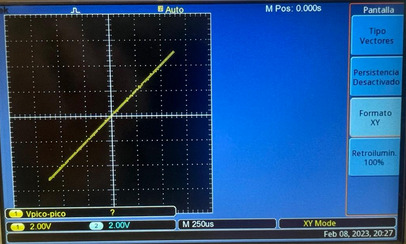
\includegraphics[scale=0.4]{Exp1_Img1.jpeg}
    \caption{Esta es la primera figura de Lissajous que encontramos, es una linea recta que se compone de dos ondas que tienen la misma amplitud y frecuencia pero que difieren en su fase inicial, en particular se difieren por $33^\circ$}
    \label{fig:Recta}
\end{figure}

\begin{figure}[H]
    \centering
    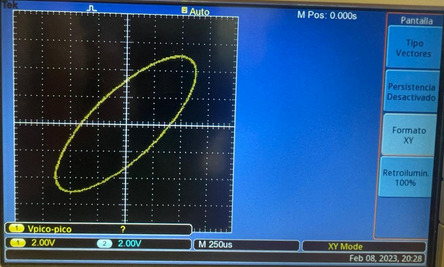
\includegraphics[scale=0.4]{Exp1_Img2.jpeg}
    \caption{Esta es la segunda figura de Lissajous que encontramos, es una elipse que se compone de dos ondas que tienen la misma amplitud y frecuencia pero que difieren en su fase inicial, en particular se difiere por $73^\circ$}
    \label{fig:Elipse}
\end{figure}

\begin{figure}
    \centering
    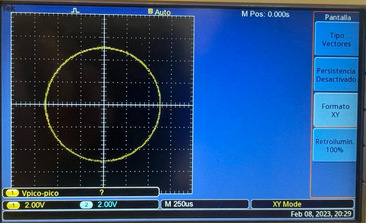
\includegraphics[scale=0.5]{Exp1_Img3.jpeg}
    \caption{Esta es la segunda figura de Lissajous que encontramos, es una esfera que se compone de dos ondas que tiene la misma amplitud y frecuencia pero que difieren en su fase inicial, en particular se difiere por $123^\circ$}
    \label{fig:Circulo}
\end{figure}
\begin{center}
    \begin{tabular}{|c|c|c|}
        \hline
        Figura & Frecuencia (Hz) & Fase Inicial ($^\circ$)\\
        \hline
        Figura \ref{fig:Recta} & 600 & 33\\
        Figura \ref{fig:Recta} & 600 & 0\\
        Figura \ref{fig:Elipse} & 600 & 73\\
        Figura \ref{fig:Elipse} & 600 & 0\\
        Figura \ref{fig:Circulo} & 600 & 123\\
        Figura \ref{fig:Circulo} & 100 & 0\\
        \hline
    \end{tabular}
\end{center}
\subsection{Experimento 2}
Los datos tomados nos presentaron varias figuras de Lissajous, estas estan en las siguientes figuras
\begin{figure}[H]
    \centering
    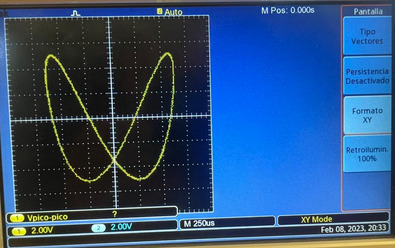
\includegraphics[scale=0.4]{Exp2_Img1.jpeg}
    \caption{Esta es una fígura de Lissajous que obtuvo con datos de frecuencia en relación 1:2 y que mantiene una fase de $33^\circ$}
    \label{fig:1_2}
\end{figure}
\begin{figure}[H]
    \centering
    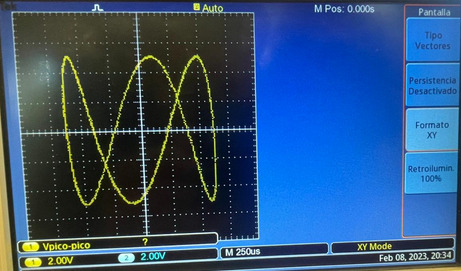
\includegraphics[scale=0.4]{Exp2_Img2.jpeg}
    \caption{Esta es una fígura de Lissajous que obtuvo con datos de frecuencia en relación 1:3 y que mantiene una fase de $33^\circ$}
    \label{fig:1_3}
\end{figure}
\begin{figure}[H]
    \centering
    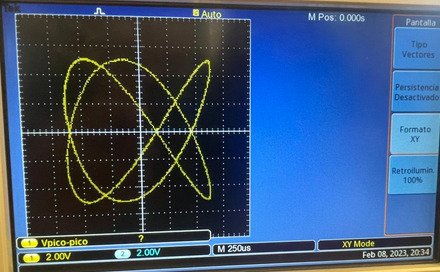
\includegraphics[scale=0.4]{Exp2_Img3.jpeg}
    \caption{Esta es una fígura de Lissajous que obtuvo con datos de frecuencia en relación 2:3 y que mantiene una fase de $33^\circ$}
    \label{fig:2_3}
\end{figure}
\begin{figure}[H]
    \centering
    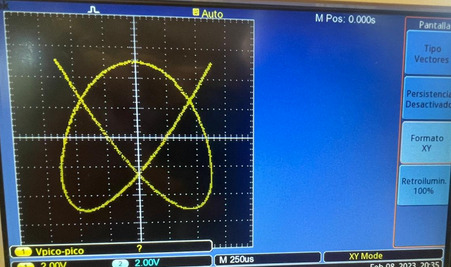
\includegraphics[scale=0.4]{Exp2_Img4.jpeg}
    \caption{Esta es una fígura de Lissajous que obtuvo con datos de frecuencia en relación 3:4 y que mantiene una fase de $33^\circ$}
    \label{fig:3_4}
\end{figure}
\begin{figure}[H]
    \centering
    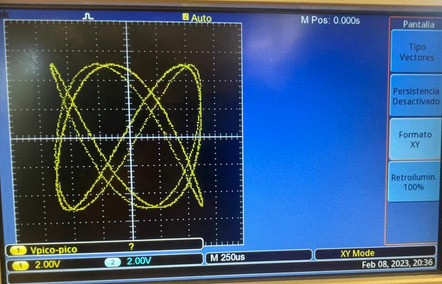
\includegraphics[scale=0.4]{Exp2_Img5.jpeg}
    \caption{Esta es una fígura de Lissajous que obtuvo con datos de frecuencia en relación 3:5 y que mantiene una fase de $33^\circ$}
    \label{fig:3_5}
\end{figure}
\begin{figure}[H]
    \centering
    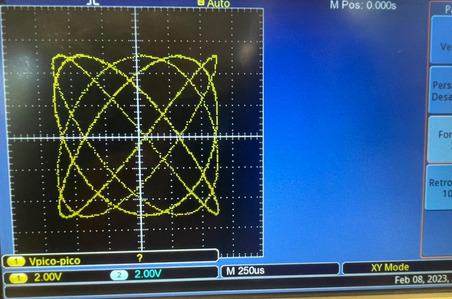
\includegraphics[scale=0.4]{Exp2_Img6.jpeg}
    \caption{Esta es una fígura de Lissajous que obtuvo con datos de frecuencia en relación 4:5 y que mantiene una fase de $33^\circ$}
    \label{fig:4_5}
\end{figure}
\begin{figure}[H]
    \centering
    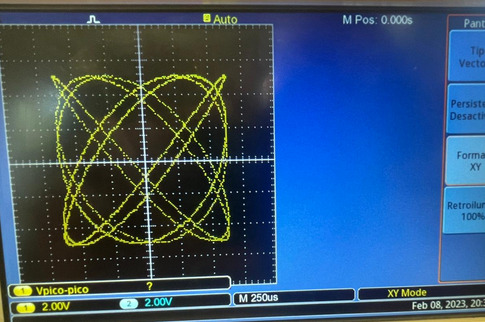
\includegraphics[scale=0.4]{Exp2_Img7.jpeg}
    \caption{Esta es una fígura de Lissajous que obtuvo con datos de frecuencia en relación 5:6 y que mantiene una fase de $33^\circ$}
    \label{fig:5_6}
\end{figure}

\begin{center}
    \begin{tabular}{|c|c|c|}
        \hline
        Figura & Frecuencia (Hz) & Fase Inicial($^\circ$)\\
        \hline
        Figura \ref{fig:1_2} & 600 & 33\\
        Figura \ref{fig:1_2} & 1200 & 0\\
        Figura \ref{fig:1_3} & 600 & 33\\
        Figura \ref{fig:1_3} & 1800 & 0\\
        Figura \ref{fig:2_3} & 1200 & 33\\
        Figura \ref{fig:2_3} & 1800 & 0\\
        Figura \ref{fig:3_4} & 1800 & 33\\
        Figura \ref{fig:3_4} & 2400 & 0\\
        Figura \ref{fig:3_5} & 1800 & 33\\
        Figura \ref{fig:3_5} & 3000 & 0\\
        Figura \ref{fig:4_5} & 2400 & 33\\
        Figura \ref{fig:4_5} & 3000 & 0\\
        Figura \ref{fig:5_6} & 3000 & 33\\
        Figura \ref{fig:5_6} & 3600 & 0\\
        \hline
    \end{tabular}
\end{center}

\section{Conclusiones}

Durante esta practica se logro entender que el generador de señales periódicas es el encargado de producir las ondas sinusoidales que se superponen y grafican en el osciloscopio. Con esto, se forman las figuras de Lissajous pues por cada eje hay una onda armonica que le da sus valores. Ademas, se comprendio el proceso por el cual existen las figuras de Lissajous y como estas son dependientes de su frecuencia y de su fase inicial, mientras que la amplitud solo tiene efecto en la escala que esta toma. Por ultimo, no se logro importar las imagenes a \textit{Logger Pro} debido a las limitaciónes impuestas por los equipos de la Universidad, sin embargo, el problema fue solucionado y el conocimiento de como se realiza se obtuvo.


\bibliographystyle{abbrv}
\bibliography{Referencias}

\end{document}
